%%%%%%%%%%%%%%%%%%%%%%%%%%%%%%%%%%%%%%%%%%%%%%%%%%%%%%%%%%%%%%%%%%%%%
%
% CSCI 1430 Python Tutorial
%
% This is a LaTeX document. LaTeX is a markup language for producing
% documents. Your first task is to compile this into a PDF document.
% 
% TO COMPILE:
%  pdflatex thisfile.tex
%
% If you do not have LaTeX and need a LaTeX distribution:
% - Online tool: https://www.overleaf.com/ (Recommended)
% - Departmental machines have one installed.
% - Personal laptops (all common OS): www.latex-project.org/get/
%
% If you need help with LaTeX, please come to office hours.
% Or, there is plenty of help online:
% https://en.wikibooks.org/wiki/LaTeX
%
%
% Once compiled, please read through and play with the examples
% in Python.
%
% Good luck!
% James and the 1430 staff
%
%%%%%%%%%%%%%%%%%%%%%%%%%%%%%%%%%%%%%%%%%%%%%%%%%%%%%%%%%%%%%%%%%%%%%

\documentclass{article}

\usepackage[english]{babel}
\usepackage[utf8]{inputenc}
\usepackage[colorlinks = true,
            linkcolor = blue,
            urlcolor  = blue]{hyperref}
\usepackage[a4paper,margin=1.5in]{geometry}
\usepackage{stackengine,graphicx}
\usepackage{fancyhdr}
\usepackage{microtype}
\usepackage{times}
\usepackage{hyperref}
% A good format for python code https://github.com/olivierverdier/python-latex-highlighting
\usepackage{pythonhighlight}


\newcommand{\commJ}[1]{\textcolor{orange}{\textsc{CommentJosh}: \emph{#1}}}
\newcommand{\commG}[1]{\textcolor{blue}{\textsc{CommentPurvi}: \emph{#1}}}

\frenchspacing
\setlength{\parindent}{0cm} % Default is 15pt.
\setlength{\parskip}{0.3cm plus1mm minus1mm}

\pagestyle{fancy}
\fancyhf{}
\lhead{Python Tutorial}
\rhead{CSCI 1430}
\rfoot{\thepage}

\date{}

\title{CSCI 1430---Python Tutorial}

\author{1430 Course Staff}

\begin{document}

\maketitle
\vspace{-2cm}
\thispagestyle{fancy}

\section{Installation}

The course uses Python as our language. As software library installation and management can often be tricky, Python supports `virtual environments' which collect and isolate a set of library packages at specific version numbers. CSCI 1430 has its own virtual environment to reduce configuration issues. You can use this virtual environment on the CS department computers, or you can recreate it on your personal machine. As a development environment, the course supports Visual Studio Code, which is a free cross-platform editor with debugging support.


\subsection{Python version numbers}

(Spring 2020) The class supports Python 3.7.3, which is the version installed on the CS department machines. Our Python virtual environment uses Python 3.7.3. Our Gradescope autograder uses the same virtual environment on Python 3.7.3.

\emph{Python 2.7 is not supported by the class.}

If you are experienced with Python and virtual environments, and you can resolve your own versioning issues, then please feel free to use a more current Python version on your personal machine. But, the code that you submit still has to pass on our autograder.


\subsection{Virtual Environment}

Python with all dependencies needed for this course is already installed on the department machines. You can enable the virtual environment on department machines using the following command:
\begin{verbatim}
$ source /course/cs1430/cs1430_env/bin/activate
\end{verbatim}

Deactivate the environment by using the following command.
\begin{verbatim}
$ deactivate
\end{verbatim}

If you would like to work on your personal machine, there is a requirements.txt file \href{http://cs.brown.edu/courses/csci1430/gradescope/requirements.txt}{here}.
Once you have Python 3.7 installed (see \hyperref[sec:local]{Working Locally}), you can use this file to install all needed libraries using the following command on your local computer:
\begin{verbatim}
$ pip3 install -r requirements.txt
\end{verbatim}

Pip is a package manager that allows us to easily install Python modules. In this scenario, the above command neatly reads a list of modules from requirements.txt and installs them all in a virtual environment. If you don't already have pip installed on your computer, you can follow the instructions \href{https://pip.pypa.io/en/stable/installing/}{here}.

\subsection{Working Locally}
\label{sec:local}
First, make sure that you have the correct version of Python installed. You can get version 3.7.3 \href{https://www.python.org/downloads/release/python-373/}{here}. To check if it installed, you can run
\begin{verbatim}
$ python3.7 --version
\end{verbatim}

If you want to recreate the \texttt{cs1430\_env} to work locally on either a macOS or Linux system, you can use the \texttt{virtualenv} utility to create a new Python virtual environment.

\textbf{WARNING:} before you hand in your assignments, make sure that your project still works using the original \texttt{cs1430\_env}. Otherwise, you may lose points during grading!

If you don't already have pip installed on your computer, you can follow the instructions \href{https://pip.pypa.io/en/stable/installing/}{here}. Then, to install \texttt{virtualenv}, run the following in a new terminal session (make sure that no other virtual environments are active).
\begin{verbatim}
$ pip3 install virtualenv
\end{verbatim}

Next, navigate to a directory of your choice (this could be the directory that contains all of your cs1430 projects) and run:
\begin{verbatim}
$ virtualenv --python=python3.7 venv
\end{verbatim}

\texttt{python3.7} is the path to the Python executable that you wish to use in your virtual environment. The version of this Python executable should be at least 3.7.

The virtualenv command above creates a new directory called \texttt{venv} that contains your new virtual env. You can activate this using the following command:
\begin{verbatim}
$ source ./venv/bin/activate
\end{verbatim}

Next install the necessary packages to your virtual environment by getting the appropriate \texttt{requirements.txt} from  \href{http://cs.brown.edu/courses/csci1430/gradescope/requirements.txt}{here} and running:
\begin{verbatim}
(venv) $ pip3 install -r <path_to_requirements.txt>
\end{verbatim}

Note that this must be run while your virtual environment is activated.

Now you can treat your \texttt{venv} just like \texttt{cs1430\_env}!

Mac virtualenv users may need to refer to following section for \texttt{matplotlib} errors.

\subsection{Common Errors}
When installing the virtual environment via \texttt{pip}, if you already have Python 2.7 installed, then \texttt{pip} may refer to your Python 2.7 installation. Use \texttt{pip3} instead to refer to your Python 3.x installation.
\begin{verbatim}
$ pip3 install -r requirements.txt
\end{verbatim}
Note that, if you do not have Python 2.7 installed, then \texttt{pip3} may not exist, and simply using \texttt{pip} is sufficient.

Likewise, when running \texttt{python} with Python 2.7 installed, then this may also refer to Python 2.7 and not Python 3.x. Instead, use the \texttt{python3} command:
\begin{verbatim}
$ python3 yourfile.py
\end{verbatim}

Another error you may run into, if you're running the virtual environment on Mac OS, is something like: ``No module named '\_tkinter'''. This seems to be an issue with the matplotlib module backend. If this happens, ensure that you include the following at the top of your Python code, when importing matplotlib.
\begin{python}
import matplotlib
matplotlib.use("TkAgg") # To run the virtual environment on MacOS. Otherwise, skip!
import matplotlib.pyplot as plt
\end{python}

\subsection{VS Code}
VS Code is a GUI-based text editor and development environment. VS Code is already installed on departmental machines. After starting it, make sure to set ``Python.VenvPath'' to \texttt{/course/cs1430/} in your VS Code settings so that it can correctly detect our custom python virtual environment. You can open the settings window with Cmd + "," (Mac) or Ctrl + "," (Windows).

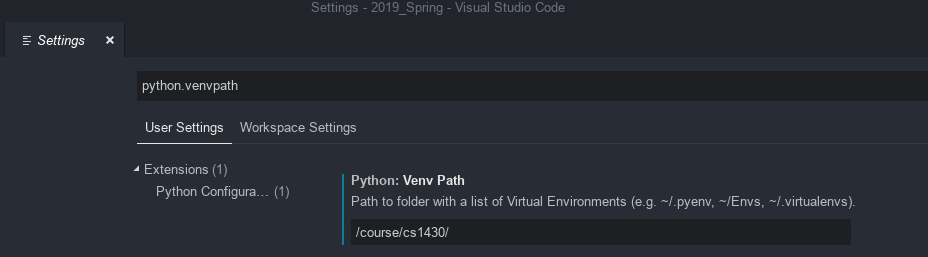
\includegraphics[width=\linewidth]{VenvPath.png}

Then, restart vscode. Once done, open a Python file, look to the bottom right, and click the `Python x.x.x' button. A list of Python environments installed on your machine should appear---select the `cs1430\_env' one. Once done, it should look like this:

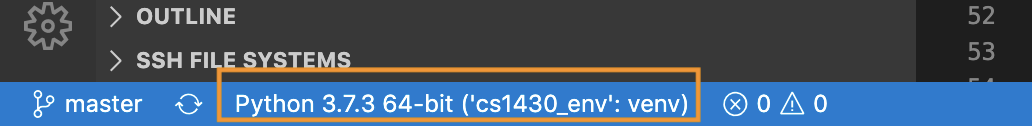
\includegraphics[width=\linewidth]{VSCode_VenvCorrect.png}

For personal laptops, please install VS Code from official Microsoft download page:\\ \href{https://code.visualstudio.com/}{https://code.visualstudio.com/}. Install the official Python extension from within VS Code (menu `View' then `Extensions', then search for `python') to allow code highlighting and debugging. Make sure to set ``Python.VenvPath'' in settings to the location where you recreated the CSCI 1430 virtual environment.


\subsection{Optional: Easier Virtual Environment Activation}
\label{sec:venvactivation}

You may wish to create an alias for the environment activation command to make it easier to type and remember. To do this, open your \texttt{.bashrc} file (located in your home directory) and enter the following at the bottom:
\begin{verbatim}
alias cs1430_env="source /course/cs1430/cs1430_env/bin/activate"
\end{verbatim}

Note that the \texttt{.bashrc} file may be hidden from the file explorer depending on your settings, but can still be opened with a command-line text editor like \texttt{nano}. The alias will not take effect until you restart (close and open) the terminal.

\section{Official Python Introduction}
If you are new to Python, we recommend starting with official introduction to Python programming:\\
\href{https://docs.python.org/3/tutorial/}{https://docs.python.org/3/tutorial/}

In general, Python's documentation is excellent, so use it liberally.:\\
\href{https://docs.python.org/3/index.html}{https://docs.python.org/3/index.html}

The rest of this document contains concepts we will assume you know. Please become familiar with them, try them out, and let us know if you have any questions.


\section{NumPy Introduction}
NumPy makes manipulating matrices and vectors in python significantly easier and faster.
If you are new to NumPy, we recommend starting with this introduction to programming with NumPy:\\
\href{https://engineering.ucsb.edu/~shell/che210d/numpy.pdf}{https://engineering.ucsb.edu/~shell/che210d/numpy.pdf}


\section{Syntax}
\subsection{Whitespace}
Please be aware of whitespace rules! Python doesn't require brackets to separate methods and classes; control flow is instead declared with indentation. The following code sample will not work, due to the indentation error in the if statement code block.
\begin{python}
x = 1
y = 2
if x < y:
x=3 # indentation error!
\end{python}
but this one will:
\begin{python}
x = 1
y = 2
if x < y:
    x=3 # Fixed by adding whitespace!
\end{python}
Indentation level is usually either indicated by a tab, or by 4 spaces. We can debate about which is better, but all that really matters is that your choice is consistent.


\section{Arrays}
\subsection{Python Lists vs.~NumPy Arrays}
Python lists and NumPy arrays are two different data structures. A Python list can contain multiple data types, whereas all elements of a NumPy array must be the same data type. NumPy arrays must be pre-allocated, whereas Python lists do not need pre-allocation. NumPy arrays can be used in vector or matrix multiplication and other linear algebra operations, whereas Python lists cannot. Note that you can convert from Python lists to NumPy arrays and vice versa, but we recommend doing so as little as possible since doing so incurs a computational overhead.

\subsection{Indexing}
To access or modify the first element of an array, the element at position 0 in the array is called. To see how this works, try the following exercise.
In a Python interpreter, create a 5-element array $A$, with integers 1 through 5 as follows:
\begin{python}
import numpy as np
A = np.arange(1, 6)
\end{python}

$A$ should now be equal to the array $[1,2,3,4,5]$.
Now, type $A[0]$ into the command window and press enter. Note that $1$ is the return value.
Now try modifying the first element of the array by setting its value to 5; type $A[1]=5$ into the command window and press enter. The value of the array should now be $[5,2,3,4,5]$.

\section{Reading and Displaying Images}
The \href{hhttp://scikit-image.org/docs/dev/api/skimage.io.html#skimage.io.imread}{$skimage.io.imread$} function is used to load images.
The \href{https://matplotlib.org/api/_as_gen/matplotlib.pyplot.imshow.html}{$matplotlib.pyplot.imshow$} function takes in a NumPy array representation of an image as a parameter and displays the image.

\subsection{Types}
There is no type declaration in Python; the language handles this automatically. However, NumPy arrays \textit{do} have types listed \href{https://docs.scipy.org/doc/numpy/user/basics.types.html}{here}, and it is critical to understand how this works to use various image processing functions.
Try downloading an image from the internet and reading it like so:
\begin{python}
from skimage import io
image = io.imread('yourimage.jpg')
\end{python}

The variable \texttt{image} now contains the color information of `yourimage.jpg' within a numpy array. If your chosen image has color, this array will be of size (height, width, 3), the 3 representing the 3 color channels. Try printing out one of the values in the array (ex: print(image[200,35,1]). You should notice that it consists of integers from 0 to 255.

At times, you will want to alter the image in ways such that some of the entries become non-integer values, and thus you will want to convert the image to floating point format by using the numpy function. You might find it tempting to cast types using \href{https://docs.scipy.org/doc/numpy-1.15.0/reference/generated/numpy.ndarray.astype.html}{$astype$}. However, astype() violates typical assumptions made \emph{in other functions} about data type ranges, and this can lead to confusion when using built-in scikit-image processing functions.

For example, when using \texttt{matplotlib.pyplot.imshow}, Matplotlib assumes that the image pixel values are between 0 and 255 if the image is in integer format; if the image is in floating-point format, it is assumed that the pixel values are in between 0 and 1. Thus, as a general rule, when you convert an image to floating-point format, you should normalize the image so that all its entries are between 0 and 1; this helps prevent potential confusion.

This is easiest done by using particular scikit-image functions that will convert safely between datatypes:
\href{http://scikit-image.org/docs/dev/api/skimage.html#skimage.img_as_float32}{$img\_as\_float32$} to go from 8-bit unsigned byte [0,255] to 32-bit floating point; this function converts an array to floating-point format and then normalizes the array so that all of its values are between 0 and 1. OR, use \href{http://scikit-image.org/docs/dev/api/skimage.html#skimage.img_as_ubyte}{$img\_as\_ubyte$} to go the other way: from a floating point [0,1] image back to an 8-bit unsigned byte [0,255]. For instance, to convert just before saving an image to disk.

You can read more about this issue \href{http://scikit-image.org/docs/dev/user_guide/data_types.html}{here}.

To illustrate these concepts, try using these functions yourself.
First, try to cast the image that you read from a file to floating-point format using \texttt{astype()} and displaying it as follows.\\
\begin{python}
import matplotlib
matplotlib.use("TkAgg") #You'll need this line if you're running the virtual environment on MacOS. Otherwise, feel free to skip it!
import matplotlib.pyplot as plt
import numpy as np
from skimage import io
image = io.imread('myimage.jpg')
image = image.astype(np.float32)
plt.imshow(image)
plt.show()
\end{python}

The displayed image should look very strange; it should hardly resemble an image. This is because it has not been normalized.
Now, try converting the image to floating-point format and normalize it from 0 to 1; then display the image:
\begin{python}
from skimage import img_as_float
image = io.imread('myimage.jpg')
floatImage = img_as_float32(image)
plt.imshow(floatImage)
plt.show()
\end{python}

The displayed image should now look normal. Also, note that if you examine any of the entries in the floatImage array, you should find that all entries have values between 0 and 1.

If ever you want to know the type of a numpy array, you can look at the `dtype' variable of the array, e.g., \texttt{print(a.dtype)}.

\emph{Note:} The \texttt{img\_as\_float} function will covert to a double-wide 64-bit floating point number (also called a float64). scikit-image provides the function \texttt{img\_as\_float32} to convert to the more efficient single-wide 32-bit floating point number (float32) format.

\subsection{Multidimensional Arrays / Matrices}
Multidimensional arrays in Numpy are an extension of the two-dimensional matrix. One of the most common usages of multidimensional arrays in computer vision is to represent images with multiple channels. For instance, an RGB image has three channels, and can be represented as a 3-D array. Each of these channels can be accessed independently.
Let us create an RGB image. To begin, let us create a 300x400x3 array and initialize it to zeros. This can be done as follows:
\begin{python}
import numpy as np
image = np.zeros((300, 400, 3))
\end{python}

Now, we assign a mid red to the first hundred columns and a bright red to the following hundred columns:
\begin{python}
image[:,0:100,0] = 0.5 # 'half' red
image[:,100:200,0] = 1 # 'full' red
\end{python}

The colon `:' indexes all elements in a particular dimension.
Finally, we can assign green randomly to the first 100 rows:
\begin{python}
image[0:100,:,2] = np.random.randint(2, size=(100,400))
# choose random integer in range [0,2)
\end{python}

To view the image, type the following into the command window:
\begin{python}
import matplotlib.pyplot as plt
plt.imshow(image)
plt.show()
\end{python}

\subsection{Color images vs.~Grayscale}
Color images are often built of several stacked color channels, each of them representing value levels of the given channel. For example, RGB images are composed of three independent channels for red, green and blue primary color components. In contrast, a grayscale image (aka black and white image) is one in which the value of each pixel is a single sample, that is, it carries only intensity information.

In Python, it is easy to convert an RGB image to grayscale. This can be achieved using scikit-image's \href{http://scikit-image.org/docs/stable/api/skimage.color.html#rgb2gray}{$rgb2gray$} function.

We can also access individual color channels of a color image. This is illustrated in the code snippet below.
\begin{python}
# Read in original RGB image.
import numpy as np
from skimage import io, color
import matplotlib.pyplot as plt
rgbImage = io.imread('yourimage.jpg')
(m,n,o) = rgbImage.shape
# Extract color channels.
redChannel = rgbImage[:,:,0] # Red channel
greenChannel = rgbImage[:,:,1] # Green channel
blueChannel = rgbImage[:,:,2] # Blue channel
# Create an all black channel.
allBlack = np.zeros((m, n), dtype=np.uint8)
# Create color versions of the individual color channels.
justRed = np.stack((redChannel, allBlack, allBlack), axis=2)
justGreen = np.stack((allBlack, greenChannel, allBlack),axis=2)
justBlue = np.stack((allBlack, allBlack, blueChannel),axis=2)
# Recombine the individual color channels to create the original RGB image again.
recombinedRGBImage = np.stack(( redChannel, greenChannel, blueChannel),axis=2)
plt.imshow(recominedRGBImage)
plt.show()
\end{python}

Try to view the various results using \href{https://matplotlib.org/api/_as_gen/matplotlib.pyplot.imshow.html}{$imshow$}. You may have to call matplotlib.pyplot.imshow(image) first, followed by matplotlib.pyplot.show(). See the above code block for an example.


\section{Performance Improvements}
Since NumPy is an extension for Python that is written in C, NumPy operations are faster than their corresponding Python equivalents. For example, performing matrix multiplication of two NumPy arrays is faster than iterating through two Python lists representing arrays and multiplying the correct elements. As such, we recommend doing as much of your calculations in NumPy as possible.
It is best to avoid using for loops whenever possible; one can attain significant performance improvements through vectorization and logical indexing.

\subsection{Pre-allocation}
Numpy does not support dynamic array allocation; it is necessary to allocate space for an array before making assignments. For example, suppose you want to create a 10 element array such that every element is the integer 5. This could be done as follows:
\begin{python}
import numpy as np
A = np.zeros(10)
for i in range(10):
    A[i]=5
\end{python}

As we can see, the array A must be initialized with 10 elements before we can change those elements. To increase the size of the array, we can use methods like numpy.append().
\begin{python}
import numpy as np
A = np.array([5]) # create an array that is too small...
for i in range(9):
    A = np.append(A, [5]) # ...that we resize every time
\end{python}

However, when using resizing methods like append() instead of pre-allocation, elements need to be re-copied every time the size of the array is increased. For a small list like this, the impact is not noticeable, but for long lists it will quickly become a bottleneck. Thus, you should always pre-allocate if possible.

\subsection{Vectors as function parameters}
Most Numpy functions support passing vectors or matrices as parameters. This prevents you having to apply the function to individual elements as a way of improving performance. It is best illustrated with a few examples:
Suppose you have a 10-element array $A$. You want to take the sine of each element and store the results in another array $B$. A naive method would use a for loop as follows:
\begin{python}
import numpy as np
B=np.zeros(10)
for i in range(10):
    B[i]=np.sin(A[i])
\end{python}

The same operation can be accomplished as follows:
\begin{python}
B=np.sin(A)
\end{python}

Similar operations can be completed if one wishes to raise every element in $A$ to a certain power. For example, suppose we want to square every element in $A$ and store the result in $B$. This can be done as follows:
\begin{python}
import numpy as np
B=np.power(A,2)
\end{python}

\subsection{Logical Indexing}
Suppose we have an $m \times n$ 2D array, and we want to set every element in the array that has a value greater than 100 to 255. This can be done as follows with a for loop:
\begin{python}
import numpy as np
import matplotlib.pyplot as plt
m = 400
n = 400
A = np.random.randint( 255, size=(m,n))
for i in range(m):
    for j in range(n):
        if A[i,j] > 100:
            A[i,j] = 255
plt.imshow( A );
plt.show()
\end{python}

A more efficient method uses logical indexing:
\begin{python}
B = A > 100
A[B] = 255
\end{python}

$B$ is now a binary logical array, where for all $i,j$, $B[i][j]=1$ if and only if $A[i][j]) > 100$; otherwise, $B[i][j]=0$. Then we do the following: $A[B] = 255$. An element-wise assignment is then performed; the result of $A$ the same as it would be using the for loop method. A appears brighter, as more pixels are set to their maximum value. Of course, removing the temporary variable $A[A > 100] = 255$ will work just as well.

\emph{Note:} Logical indexing also works across multi-channel images! Even though we can split out each of our color channels and index into them individually, we can also logically index directly into the three-channel RGB image.

\subsection{Evaluating Performance}
We can evaluate time performance using the Python package time. It is used as follows:
\begin{python}
import time
start = time.time()
# Perform some operation
end = time.time()
print(end - start)
\end{python}

The elapsed time between the variables start and end is then printed out. You should try doing several of the examples above, and note the performance differences between using for loops and using the more efficient methods.


\section{Debugging}
\label{sec:debugger}
There are a few debuggers that exist for Python. We support using VS Code with the Python extension.
To use this debugger, download the Python extension from the following page: \href{https://marketplace.visualstudio.com/items?itemName=ms-python.python}{https://marketplace.visualstudio.com/items?itemName=ms-python.python}. This extension also provides linting (syntax checking) and autocomplete.

Please see the following VS Code page for information on how to enter the debugger, and how to set and navigate breakpoints:
\href{https://code.visualstudio.com/docs/editor/debugging}{VS Code Debugger}

VS Code should automatically detect the configuration and run properly when you press ``F5'' when editing your main file. If it does not work, check the version of python that VS Code has selected by looking at the bottom left corner. It should be the ``cs1430\_env'' virtualenvironment. You can change the version by clicking on version displayed in the bottom left and selecting a different version using the drop down menu. If this setup does not work, please come to TA hours.

\section{Project 0 questions}
Made it this far? Good. Now, please attempt the three Project 0 questions on the course Webpage.

\end{document}
